\section{Introduction}

Culture and language are closely intertwined.
As a result, different countries speaking the same language, e.g.,
US and UK, may demonstrate subtle differences in the usage
of the language.
For example, football may refer to American football in one country
and soccer in another.
Unawareness of such difference often leads to a misunderstanding,
to avoid which there have been manual annotations in major dictionaries
on cultural difference (see \figref{fig:ox} and \figref{fig:wiki}).

\begin{figure}[h]
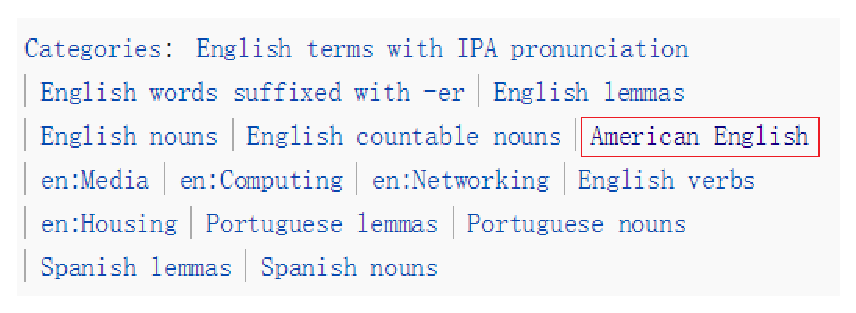
\includegraphics[width=0.9\linewidth]{img/wiki}
\caption{Wiktionary categories of ``trailer''}
\label{fig:wiki}
\end{figure}

\begin{figure}[h]
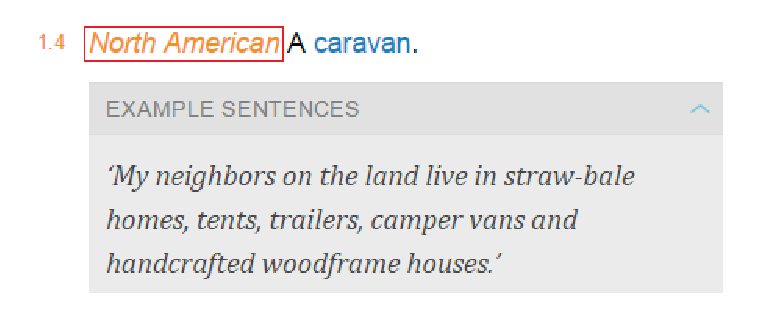
\includegraphics[width=0.9\linewidth]{img/oxford}
\caption{Oxford Dictionary entry of ``trailer''}
\label{fig:ox}
\end{figure}

The goal of this paper is to automatically build such annotations.
Manual annotation is inherently limited to popular words in the two
cultures, and cannot scale well to new or rare words.
In contrast, we seek to automatically mine cultural difference annotations
from large corpora. Existing work has focused on mining
synonymous word pairs across
different languages\cite{Mikolov:2013tp}, or bilingual lexicon\cite{linard2015bilingual}, for translation.
While mining bilingual lexicon has been actively studied,
mining cultural difference between countries using the same language
is yet to be done.


In particular, we learn representations from Skip-grams
as recently proposed in~\cite{Mikolov2013distributed}.
These models, using a neural network architecture,
are trained on the American and the British corpora, respectively,
such that each word is represented by two numerical vectors, one for
American use and one for British use. The semantic similarity can then
be represented by the vector similarity, after a trained linear transformation
\cite{Mikolov:2013tp} from the British English vector space
to the American one.
%As vector similarity represents semantic similarity,
%existing efforts for mining bilingual lexicon
%proposed to learn a
%transformation between
%semantically identical words from a language to another with word embedding.

We compare the results from the Skip-gram model to two other simpler
word co-ocurrence based methods as well as the random annotation and show
that the Skip-gram model outperforms the rest at significant margin
with an F1 score of 0.247 when taking the top 1000 words, 57.3\% more than
the simpler TF-IDF method.



